\documentclass[norsk,a4paper,12pt]{article}
\usepackage[utf8]{inputenc}
\usepackage{graphicx} %for å inkludere grafikk
\usepackage{verbatim} %for å inkludere filer med tegn LaTeX ikke liker
\usepackage{tabularx}
\usepackage{booktabs}
\usepackage{amsmath}
\usepackage{float}
\usepackage{listings}
\usepackage{hyperref}
%\usepackage{subfigure}
\usepackage{subcaption}
\usepackage{caption}
\usepackage{color}
\usepackage[sep=3pt, offset=0.8em]{simpler-wick}
\usepackage{tikz}

\lstset{language=python}
\lstset{basicstyle=\small}
\lstset{backgroundcolor=\color{white}}
\lstset{frame=single}
\lstset{stringstyle=\ttfamily}
\lstset{keywordstyle=\color{red}\bfseries}
\lstset{commentstyle=\itshape\color{blue}}
\lstset{showspaces=false}
\lstset{showstringspaces=false}
\lstset{showtabs=false}
\lstset{breaklines}
\lstset{postbreak=\raisebox{0ex}[0ex][0ex]{\ensuremath{\color{red}\hookrightarrow\space}}}
%\usepackage{titlesec}

\setcounter{secnumdepth}{4}


\title{FYS-KJM4480 - Quantum mechanics for many-particle systems \\\vspace{2mm} \Large{Project 2}}
\author{\large Even Marius Nordhagen}
\date\today
\begin{document}

\maketitle

\begin{itemize}
\item For the Github repository containing programs and results, follow this link: 
\url{https://github.com/evenmn/master/tree/master/FYSKJM4480/Project2}
\end{itemize}

\section*{Introduction}
Superconductivity might be one of 20th century's most exciting physical discoveries, and for a long time the theory behind was a mystery. In 1957, 46 years after the first observation by Kamerlingh Onnes [REFERENCE], John Bardeen, Leon Cooper and John Robert Schrieffer came up with a quantum theory describing superconductivity on microscopic level[REFERENCE]. This theory was built on Cooper pairs, which is a pair of electrons with lower energy than the Fermi energy, i.e. there is a bounding between them. We can treat the pairs as a spinless particle, which is a boson, and this boson-like pair is the reason why the current can flow unhindered in a superconductor. 

Furthermore the theory is also used in nuclear physics to describe the paring interaction between nucleons in an atomic nucleus. 

This project aims to study such a pairing model, known as BCS-theory after its founders. In the first part we are working with this model independently. Then we will use Full Configuration-Interaction (FCI) to find the exact energy eigenvalues, and Configuration-Interaction Doubles (CID) and Rayleigh-Schrodinger Perturbation Theory of third order (RSPT3) as approximations to increase the performance. Thereafter we repeat this using Coupled-Cluster Doubled (CCD), and finally we compare all the approximations to the exact solutions.
\newpage

\section{Pairing model}
In this project we use a slightly simplified pairing model, which we assume to be carrying a constant strength $g$. The Hamiltonian is therefore given by
\begin{equation}
\hat{H}=\hat{H}_0+\hat{V}
\end{equation}
with
\begin{equation}
\hat{H}_0=\sum_{p\sigma}\epsilon_pc_{p\sigma}^{\dagger}c_{p\sigma},\quad \epsilon_p=\xi\cdot(p-1)
\label{eq:H0_init}
\end{equation}
and
\begin{equation}
\hat{V}=-\frac{1}{2}g\sum_{pq}c_{p+}^{\dagger}c_{p-}^{\dagger}c_{q-}c_{q+}.
\label{eq:V_init}
\end{equation}
where $\epsilon_p=\xi(p-1)$, with $\xi$ set to 1.

We will only study systems of a even number of particles, $N$, and the ground-state wavefunction is then given by the Slater determinant
\begin{equation}
|\Phi\rangle=c_{1+}^{\dagger}c_{1-}^{\dagger}\hdots c_{N/2 +}^{\dagger}c_{N/2 -}^{\dagger}|\Phi\rangle.
\end{equation}
Further I will define some operators that will be useful when doing the calculations. 
\begin{equation}
\hat{P}_p^{\dagger}\equiv c_{p+}^{\dagger}c_{p-}^{\dagger},\quad \hat{P}_p\equiv c_{p-}c_{p+}
\end{equation}
\begin{equation}
\hat{n}_p\equiv\sum_{\sigma}c_{p\sigma}^{\dagger}c_{p\sigma}
\end{equation}
\begin{equation}
\hat{P}=\sum_p\hat{P}_p^{\dagger}\hat{P}_p
\end{equation}
and finally
\begin{equation}
\hat{S}_z=\frac{1}{2}\sum_{p\sigma}\sigma c_{p\sigma}^{\dagger}c_{p\sigma}.
\end{equation}

If $\hat{H}$, $\hat{P}$ and $\hat{S}_z$ commute, we can reduce this problem to an eigenvalue problem on the form
\begin{align*}
\hat{H}|\Psi_k;S_z,P\rangle&=E_{k,S_z,P}|\Psi_k;S_z,P\rangle\\
\hat{P}|\Psi_k;S_z,P\rangle&=P|\Psi_k;S_z,P\rangle\\
\hat{S}_z|\Psi_k;S_z,P\rangle&=S_z|\Psi_k;S_z,P\rangle
\end{align*}
where the eigenvalues are the energies, the number of pairs and the spin in z-direction respectively. We need to check this:

\subsection*{1A}
Firstly, we check if the Hamiltonian commutes with the spin-projection operator, and since $\hat{H}=\hat{H}_0+\hat{V}$, we can split this calculation into two simpler calculations. Let us start with $[\hat{H}_0,\hat{S}_z]$:
\begin{align*}
[\hat{H}_0,\hat{S}_z]&=\bigg[\sum_{p\sigma}\epsilon_pc_{p\sigma}^{\dagger}c_{p\sigma},\frac{1}{2}\sum_{q\sigma}\sigma c_{q\sigma}^{\dagger}c_{q\sigma}\bigg]\notag\\
&=\frac{1}{2}\sum_{pq\sigma}\epsilon_{p}\sigma(c_{p\sigma}^{\dagger}c_{p\sigma}c_{q\sigma}^{\dagger}c_{q\sigma}-c_{q\sigma}^{\dagger}c_{q\sigma}c_{p\sigma}^{\dagger}c_{p\sigma})
\end{align*}
We use Wick's theorem on the two terms, and observe that only single contraction will contribute because of the orientation
\begin{equation*}
c_{p\sigma}^{\dagger}c_{p\sigma}c_{q\sigma}^{\dagger}c_{q\sigma}=\{c_{p\sigma}^{\dagger}c_{q\sigma}^{\dagger}c_{p\sigma}c_{q\sigma}\}+\delta_{pq}c_{p\sigma}^{\dagger}c_{q\sigma}
\end{equation*}
\begin{equation*}
c_{q\sigma}^{\dagger}c_{q\sigma}c_{p\sigma}^{\dagger}c_{p\sigma}=\{c_{p\sigma}^{\dagger}c_{q\sigma}^{\dagger}c_{p\sigma}c_{q\sigma}\}+\delta_{qp}c_{q\sigma}^{\dagger}c_{p\sigma}
\end{equation*}
The first terms (the normal-ordered products) cancel, and we obtain
\begin{equation*}
[\hat{H}_0,\hat{S}_z]=\frac{1}{2}\sum_{pq\sigma}\epsilon_p\sigma(\delta_{pq}c_{p\sigma}^{\dagger}c_{q\sigma}-\delta_{qp}c_{q\sigma}^{\dagger}c_{p\sigma})
\end{equation*}
We get contribution only when $q=p$
\begin{equation*}
[\hat{H}_0,\hat{S}_z]=\frac{1}{2}\sum_{p\sigma}\epsilon_p(c_{p\sigma}^{\dagger}c_{p\sigma}-c_{p\sigma}^{\dagger}c_{p\sigma})=0
\end{equation*}

So $\hat{H}_0$ commutes with the spin-projection operator. Further we need to work out  $[\hat{V},\hat{S}_z]$:
\begin{align*}
[\hat{V},\hat{S}_z]&=\bigg[-\frac{1}{2}g\sum_{pq}c_{p+}^{\dagger}c_{p-}^{\dagger}c_{q-}c_{q+},\frac{1}{2}\sum_{r\sigma}\sigma c_{r\sigma}^{\dagger}c_{r\sigma}\bigg]\notag\\
&=-\frac{1}{4}\sum_{pqr\sigma}\sigma(c_{p+}^{\dagger}c_{p-}^{\dagger}c_{q-}c_{q+}c_{r\sigma}^{\dagger}c_{r\sigma}-c_{r\sigma}^{\dagger}c_{r\sigma}c_{p+}^{\dagger}c_{p-}^{\dagger}c_{q-}c_{q+})
\end{align*}
The fours terms written out are as follows
\begin{equation*}
c_{p+}^{\dagger}c_{p-}^{\dagger}c_{q-}c_{q+}c_{r+}^{\dagger}c_{r+}=\{c_{p+}^{\dagger}c_{p-}^{\dagger}c_{r+}^{\dagger}c_{q-}c_{q+}c_{r+}\}+\delta_{qr}c_{p+}^{\dagger}c_{p-}^{\dagger}c_{q-}c_{r+}
\end{equation*}
\begin{equation*}
c_{p+}^{\dagger}c_{p-}^{\dagger}c_{q-}c_{q+}c_{r-}^{\dagger}c_{r-}=\{c_{p+}^{\dagger}c_{p-}^{\dagger}c_{r-}^{\dagger}c_{q-}c_{q+}c_{r-}\}+\delta_{qr}c_{p+}^{\dagger}c_{p-}^{\dagger}c_{r-}c_{q+}
\end{equation*}
\begin{equation*}
c_{r+}^{\dagger}c_{r+}c_{p+}^{\dagger}c_{p-}^{\dagger}c_{q-}c_{q+}=\{c_{p+}^{\dagger}c_{p-}^{\dagger}c_{r+}^{\dagger}c_{q-}c_{q+}c_{r+}\}+\delta_{rp}c_{r+}^{\dagger}c_{p-}^{\dagger}c_{q-}c_{q+}
\end{equation*}
\begin{equation*}
c_{r-}^{\dagger}c_{r-}c_{p+}^{\dagger}c_{p-}^{\dagger}c_{q-}c_{q+}=\{c_{p+}^{\dagger}c_{p-}^{\dagger}c_{r-}^{\dagger}c_{q-}c_{q+}c_{r-}\}+\delta_{rp}c_{p+}^{\dagger}c_{r-}^{\dagger}c_{q-}c_{q+}
\end{equation*}
Again the first terms cancel, and we are left with
\begin{align*}
[\hat{V},\hat{S}_z]=-\frac{1}{4}g\sum_{pqr\sigma}\sigma\Big(&(\delta_{qr}c_{p+}^{\dagger}c_{p-}^{\dagger}c_{q-}c_{r+}+\delta_{qr}c_{p+}^{\dagger}c_{p-}^{\dagger}c_{r-}c_{q+})-\notag\\
&(\delta_{rp}c_{r+}^{\dagger}c_{p-}^{\dagger}c_{q-}c_{q+}+\delta_{rp}c_{p+}^{\dagger}c_{r-}^{\dagger}c_{q-}c_{q+})\Big)
\end{align*}
In the first two terms we will get contributions when $r=q$, and for the two last terms we will get contributions when $r=p$. We can easily see that the two first terms become equal to the two last terms, and will cancel each other.

\subsection*{1B}
Secondly, we check if the Hamiltonian commutes with the counter-operator. Again we split up:
\begin{align*}
[\hat{H}_0, \hat{P}]&=\Big[\sum_{p\sigma}\epsilon_pc_{p\sigma}^{\dagger}c_{p\sigma},\sum_q\hat{P}_q\hat{P}_q\Big]\\
&= \begin{aligned}[t]
\sum_{pq}\epsilon_p\Big[&(c_{p+}^{\dagger}c_{p+}c_{q+}^{\dagger}c_{q-}^{\dagger}c_{q-}c_{q+}
+c_{p-}^{\dagger}c_{p-}c_{q+}^{\dagger}c_{q-}^{\dagger}c_{q-}c_{q+})\\
&(c_{q+}^{\dagger}c_{q-}^{\dagger}c_{q-}c_{q+}c_{p+}^{\dagger}c_{p+}
+c_{q+}^{\dagger}c_{q-}^{\dagger}c_{q-}c_{q+}c_{p-}^{\dagger}c_{p-})\Big]
\end{aligned}
\end{align*}
We can immediately see that each term only will allow one (non-zero) contraction when Wick's theorem is used:
\begin{equation*}
c_{p+}^{\dagger}c_{p+}c_{q+}^{\dagger}c_{q-}^{\dagger}c_{q-}c_{q+}=\{c_{p+}^{\dagger}c_{q+}^{\dagger}c_{q-}^{\dagger}c_{p+}c_{q-}c_{q+}\}+\delta_{pq}c_{p+}^{\dagger}c_{q-}^{\dagger}c_{q-}c_{q+}
\end{equation*}
\begin{equation*}
c_{p-}^{\dagger}c_{p-}c_{q+}^{\dagger}c_{q-}^{\dagger}c_{q-}c_{q+}=\{c_{p-}^{\dagger}c_{q+}^{\dagger}c_{q-}^{\dagger}c_{p-}c_{q-}c_{q+}\}-\delta_{pq}c_{p-}^{\dagger}c_{q+}^{\dagger}c_{q-}c_{q+}
\end{equation*}
\begin{equation*}
c_{q+}c_{q-}c_{p+}^{\dagger}c_{p+}c_{q+}^{\dagger}c_{q-}^{\dagger}=\{c_{p+}^{\dagger}c_{q+}^{\dagger}c_{q-}^{\dagger}c_{p+}c_{q-}c_{q+}\}+\delta_{qp}c_{q+}^{\dagger}c_{q-}^{\dagger}c_{q-}c_{p+}
\end{equation*}
\begin{equation*}
c_{q+}c_{q-}c_{p-}^{\dagger}c_{p-}c_{q+}^{\dagger}c_{q-}^{\dagger}=\{c_{p-}^{\dagger}c_{q+}^{\dagger}c_{q-}^{\dagger}c_{p-}c_{q-}c_{q+}\}-\delta_{qp}c_{q-}^{\dagger}c_{q+}^{\dagger}c_{p-}c_{q+}
\end{equation*}
Recall that we sum over all possible $p$ and $q$s, and for each $p$ we will have a $q$ which is equal. Due to the Kronecker delta, we only get contributions when this happens ($p=q$), but a watchful eye will see that the terms cancel in this case $\Rightarrow [\hat{H}_0,\hat{P}]=0$.



\subsection*{1C}
The last commutator we need to check is $[\hat{P},\hat{S}_z]$:
\begin{align*}
[\hat{P},\hat{S}_z]&=[\sum_p\hat{P}_p^{\dagger}\hat{P}_p,\frac{1}{2}\sum_{q\sigma}\sigma c_{q\sigma}^{\dagger}c_{q\sigma}]\notag\\
&=\frac{1}{2}\sum_{pq\sigma}\sigma[\hat{P}_p^{\dagger}\hat{P}_p,c_{q\sigma}^{\dagger}c_{q\sigma}]\notag\\
&=\frac{1}{2}\sum_{pq}\Big(+(c_{p+}^{\dagger}c_{p-}^{\dagger}c_{p-}c_{p+}c_{q+}^{\dagger}c_{q+}-c_{q+}^{\dagger}c_{q+}c_{p+}^{\dagger}c_{p-}^{\dagger}c_{p-}c_{p+})\notag\\
&\mathrel{\phantom{=}}-(c_{p+}^{\dagger}c_{p-}^{\dagger}c_{p-}c_{p+}c_{q-}^{\dagger}c_{q-}-c_{q-}^{\dagger}c_{q-}c_{p+}^{\dagger}c_{p-}^{\dagger}c_{p-}c_{p+})\Big)
\end{align*}
We get four terms, which will be worked out separately:
\begin{equation*}
c_{p+}^{\dagger}c_{p-}^{\dagger}c_{p-}c_{p+}c_{q+}^{\dagger}c_{q+} = \{c_{p+}^{\dagger}c_{p-}^{\dagger}c_{q+}^{\dagger}c_{q+}c_{p-}c_{p+}\}+\delta_{pq}c_{p+}^{\dagger}c_{p-}^{\dagger}c_{p-}c_{q+}
\end{equation*}
\begin{equation*}
c_{q+}^{\dagger}c_{q+}c_{p+}^{\dagger}c_{p-}^{\dagger}c_{p-}c_{p+} = \{c_{p+}^{\dagger}c_{p-}^{\dagger}c_{q+}^{\dagger}c_{q+}c_{p-}c_{p+}\}+\delta_{qp}c_{q+}^{\dagger}c_{p-}^{\dagger}c_{p-}c_{p+}
\end{equation*}
\begin{equation*}
c_{p+}^{\dagger}c_{p-}^{\dagger}c_{p-}c_{p+}c_{q-}^{\dagger}c_{q-} = \{c_{p+}^{\dagger}c_{p-}^{\dagger}c_{q-}^{\dagger}c_{q-}c_{p-}c_{p+}\}-\delta_{pq}c_{p+}^{\dagger}c_{p-}^{\dagger}c_{p+}c_{q-}
\end{equation*}
\begin{equation*}
c_{q-}^{\dagger}c_{q-}c_{p+}^{\dagger}c_{p-}^{\dagger}c_{p-}c_{p+} = \{c_{p+}^{\dagger}c_{p-}^{\dagger}c_{q-}^{\dagger}c_{q-}c_{p-}c_{p+}\}-\delta_{qp}c_{p+}^{\dagger}c_{q-}^{\dagger}c_{p+}c_{p-}
\end{equation*}
Observe that the first terms cancel, and we are left with terms of $\delta_{pq}$ and $\delta_{qp}$. Those will contribute if and only if $p=q$, which happens exactly once since both $p$ and $q$ runs over all possible states. 
\begin{align*}
[\hat{P}, \hat{S}_z]&= \begin{aligned}[t]
\frac{1}{2}\sum_p\Big(&(c_{p+}^{\dagger}c_{p-}^{\dagger}c_{p-}c_{p+}+c_{p+}^{\dagger}c_{p-}^{\dagger}c_{p+}c_{p-})-\notag\\
&(c_{p+}^{\dagger}c_{p-}^{\dagger}c_{p-}c_{p+}+c_{p+}^{\dagger}c_{p-}^{\dagger}c_{p+}c_{p-})\Big)
\end{aligned}\\
&=0
\end{align*}


\subsection*{1D}
\begin{equation*}
[\hat{P}_p,\hat{P}_q^{\dagger}]=\hat{P}_p\hat{P}_q^{\dagger}-\hat{P}_q^{\dagger}\hat{P}_p
\end{equation*}
Will only include terms which contribute, and we obtain
\begin{align*}
\hat{P}_p\hat{P}_q^{\dagger}
&=c_{p-}c_{p+}c_{q+}^{\dagger}c_{q-}^{\dagger}\notag\\
&=\{c_{q+}^{\dagger}c_{q-}^{\dagger}c_{p-}c_{p+}\}+\wick{\c c_{p-}c_{p+}c_{q+}^{\dagger}\c c_{q-}^{\dagger}}+\wick{c_{p-}\c c_{p+}\c c_{q+}^{\dagger}c_{q-}^{\dagger}}+\wick{\c2 c_{p-}\c1 c_{p+}\c1 c_{q+}^{\dagger}\c2 c_{q-}^{\dagger}}\notag\\
&=\{c_{q+}^{\dagger}c_{q-}^{\dagger}c_{p-}c_{p+}\}-\delta_{pq}c_{p+}c_{q+}^{\dagger}-\delta_{pq}c_{p-}c_{q-}^{\dagger}+\delta_{pq}\delta_{pq}
\end{align*}
due to Wick's theorem. Several terms vanish since a delta function of operators of opposite spin does not contribute, i.e. $\delta_{p+q-}=0$. Calculating $\hat{P}_q^{\dagger}\hat{P}_p$ is a simple task:
\begin{equation*}
\hat{P}_q^{\dagger}\hat{P}_p=\{c_{q+}^{\dagger}c_{q-}^{\dagger}c_{p-}c_{p+}\}.
\end{equation*}
Furthermore we will omit the spin in delta functions, because it does not affect the delta function as long as the spin is equally directed. As always the deltas $\delta_{pq}$ contribute if and only if $p=q$, so we can set $q=p$ in the operators after the first delta in each term:
\begin{align}
\hat{P}_p\hat{P}_q^{\dagger}-\hat{P}_q^{\dagger}\hat{P}_p&=-\delta_{pq}c_{q+}^{\dagger}c_{q+}-\delta_{pq}c_{q-}^{\dagger}c_{q-}+\delta_{pq}\delta_{qq}\notag\\
&=\delta_{pq}(1-c_{q+}^{\dagger}c_{q+}-c_{q-}^{\dagger}c_{q-})\notag\\
&=\delta_{pq}(1-\hat{n}_q)\label{eq:ex1d}
\end{align}

\subsection*{1E}
A fundamental property of the annihilation operator states that a such operator acting on the vacuum state becomes zero. This property will be used multiple times henceforce to get rid of terms, and the approach will often be to move the annihilation operator(s) all the way to the right such that this happens. 
We have $N=4$, thus 
\begin{align*}
|\Phi\rangle&=c_{1+}^{\dagger}c_{1-}^{\dagger}c_{2+}^{\dagger}c_{2-}^{\dagger}|-\rangle\\
&=\hat{P}_1^{\dagger}\hat{P}_2^{\dagger}|-\rangle.
\end{align*}
$M$ is the number of states, with $p$ as the index
\begin{align*}
\hat{P}&=\sum_{p=1}^M\hat{P}_p^{\dagger}\hat{P}_p\\
&=\hat{P}_1^{\dagger}\hat{P}_1+\hat{P}_2^{\dagger}\hat{P}_2+\hat{P}_3^{\dagger}\hat{P}_3+\hat{P}_4^{\dagger}\hat{P}_4
\end{align*}
since $M=4$. 
\begin{align*}
\hat{P}|\Phi\rangle&=\sum_p\hat{P}_p^{\dagger}\hat{P}_p\hat{P}_1^{\dagger}\hat{P}_2^{\dagger}|-\rangle
\end{align*}
The result obtained in exercise 1D will not be used to move $\hat{P}_p$ (the only operator containing annihilation operators) to the right. 
\begin{align*}
\hat{P}|\Phi\rangle
&=\sum_p\hat{P}_p^{\dagger}\Big(\hat{P}_1^{\dagger}\hat{P}_p+\delta_{p1}(1-\hat{n}_1)\Big)\hat{P}_2^{\dagger}|-\rangle\\
&=\sum_p\hat{P}_p^{\dagger}\hat{P}_1^{\dagger}\hat{P}_p\hat{P}_2^{\dagger}|-\rangle+\sum_p\delta_{p1}\hat{P}_p^{\dagger}\hat{P}_2^{\dagger}|-\rangle+\sum_p\delta_{p1}\hat{P}_p^{\dagger}\hat{n}_1\hat{P}_2^{\dagger}|-\rangle
\end{align*}
The last term vanishes because the number operator is hermitian, and can therefore be moved to the right. The second term becomes $|\Phi\rangle$ since the delta "requires" $p=1$. We are left with the first term to work out, and again we use equation (\ref{eq:ex1d}):
\begin{align*}
\sum_p\hat{P}_p^{\dagger}\hat{P}_1^{\dagger}\hat{P}_p\hat{P}_2^{\dagger}|-\rangle
&=\sum_p\hat{P}_p^{\dagger}\hat{P}_1^{\dagger}\hat{P}_2^{\dagger}\hat{P}_p|-\rangle+\sum_p\hat{P}_p^{\dagger}\hat{P}_1^{\dagger}\delta_{p2}(1-\hat{n}_2)|-\rangle\\
&=\sum_p\delta_{p2}\hat{P}_p^{\dagger}\hat{P}_1^{\dagger}|-\rangle+\sum_p\hat{P}_p^{\dagger}\hat{P}_1^{\dagger}\hat{n}_2|-\rangle\\
&=\hat{P}_2^{\dagger}\hat{P}_1^{\dagger}|-\rangle=|\Phi\rangle
\end{align*}
On line number one the first term vanished because an annihilation operator acted on the vacuum state and on the second line the last term vanished since it contained a number operator. In total we then have:
\begin{equation}
\hat{P}|\Phi\rangle=|\Phi\rangle+|\Phi\rangle=2|\Phi\rangle
\end{equation}
The calculations above are pretty well-commented, but since the same operations are repeating, I do not consider that much comments as necessary in the coming calculations. For the $\hat{P}|\Phi\rangle$ calculation we were lucky since we could use pair creation and pair annihilation operators and could use the result from 1D. This is not always the case, something we will see when calculating $\hat{S}_z|\Phi\rangle$.
\begin{align*}
\hat{S}_z&=\frac{1}{2}\sum_{p\sigma}\sigma c_{p\sigma}^{\dagger}c_{p\sigma}\\
&=\frac{1}{2}\Big(c_{1+}^{\dagger}c_{1+}-c_{1-}^{\dagger}c_{1-}+c_{2+}^{\dagger}c_{2+}-c_{2-}^{\dagger}c_{2-}+\notag\\
&\mathrel{\phantom{=}}c_{3+}^{\dagger}c_{3+}-c_{3-}^{\dagger}c_{3-}+c_{4+}^{\dagger}c_{4+}-c_{4-}^{\dagger}c_{4-}\Big)|-\rangle
\end{align*}
\begin{align}
\hat{S}_z|\Phi\rangle
&=\frac{1}{2}\Big(c_{1+}^{\dagger}c_{1+}c_{1+}^{\dagger}c_{1-}^{\dagger}c_{2+}^{\dagger}c_{2-}^{\dagger}-c_{1-}^{\dagger}c_{1-}c_{1+}^{\dagger}c_{1-}^{\dagger}c_{2+}^{\dagger}c_{2-}^{\dagger}\notag\\
&\mathrel{\phantom{=}}+c_{2+}^{\dagger}c_{2+}c_{1+}^{\dagger}c_{1-}^{\dagger}c_{2+}^{\dagger}c_{2-}^{\dagger}-c_{2-}^{\dagger}c_{2-}c_{1+}^{\dagger}c_{1-}^{\dagger}c_{2+}^{\dagger}c_{2-}^{\dagger}\Big)|-\rangle\notag\\
&=\frac{1}{2}\Big(\wick{c_{1+}^{\dagger}\c1 c_{1+}\c1 c_{1+}^{\dagger}c_{1-}^{\dagger}c_{2+}^{\dagger}c_{2-}^{\dagger}-c_{1-}^{\dagger}\c2 c_{1-}c_{1+}^{\dagger}\c2 c_{1-}^{\dagger}c_{2+}^{\dagger}c_{2-}^{\dagger}}\notag\\
&\mathrel{\phantom{=}}+\wick{c_{2+}^{\dagger}\c3 c_{2+}c_{1+}^{\dagger}c_{1-}^{\dagger}\c3 c_{2+}^{\dagger}c_{2-}^{\dagger}-c_{2-}^{\dagger}\c4 c_{2-}c_{1+}^{\dagger}c_{1-}^{\dagger}c_{2+}^{\dagger}\c4 c_{2-}^{\dagger}}\Big)|-\rangle\notag\\
&=\frac{1}{2}\Big(\delta_{1+1+}c_{1+}^{\dagger}c_{1-}^{\dagger}c_{2+}^{\dagger}c_{2-}^{\dagger}-\delta_{1-1-}c_{1+}^{\dagger}c_{1-}^{\dagger}c_{2+}^{\dagger}c_{2-}^{\dagger}\notag\\
&\mathrel{\phantom{=}}+\delta_{2+2+}c_{1+}^{\dagger}c_{1-}^{\dagger}c_{2+}^{\dagger}c_{2-}^{\dagger}-\delta_{2-2-}c_{1+}^{\dagger}c_{1-}^{\dagger}c_{2+}^{\dagger}c_{2-}^{\dagger}\Big)|-\rangle\notag\\
&=\frac{1}{2}(1-1+1-1)|\Phi\rangle\notag\\
&=0|\Phi\rangle
\end{align}
PS: I know this was a tedious approach, and perhaps it would be better to not write out the sum

\subsection*{1F}
In the previous exercise we saw that $\hat{P}_1^{\dagger}\hat{P}_2^{\dagger}|-\rangle$ is an eigenvector of $\hat{P}$ and $\hat{S}_z$, and the basis which spans the subspace of Hilbert space should have the same form, exactly $\hat{P}_p^{\dagger}\hat{P}_q^{\dagger}|-\rangle$ Observe that $|1\bar{1}2\bar{2}\rangle=|\Phi\rangle$.

\begin{figure*}
\begin{center}
  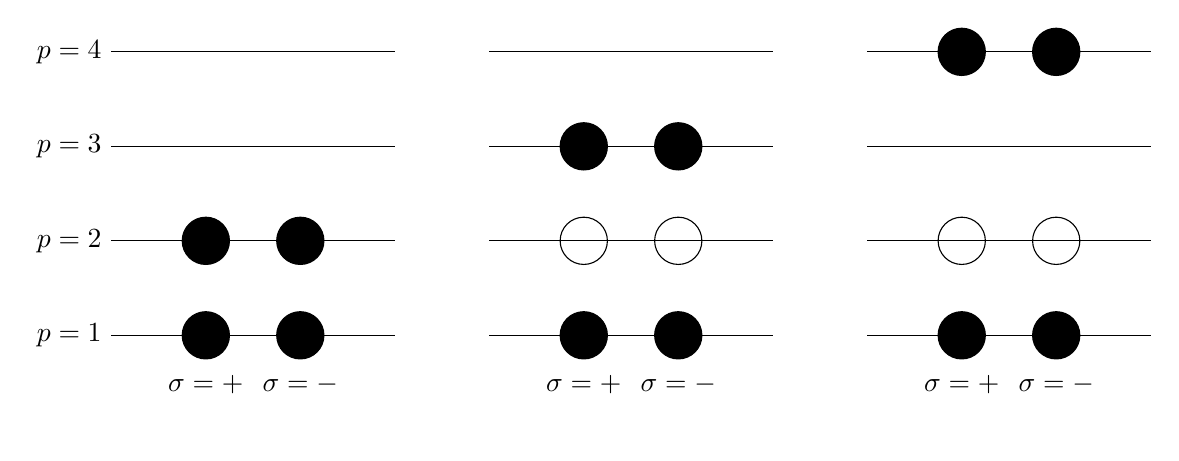
\begin{tikzpicture}[scale=1.2]
    \begin{scope}
      \foreach \i in {1,...,4}
      {
        \draw (-1,\i-1) node[anchor=east] {$p = \i$} --(2,\i-1);
      }
      \filldraw (0,0) node[anchor=north,inner sep=.5cm] {$\sigma=+$} circle (0.25cm); 
      \filldraw (1,0) node[anchor=north,inner sep=.5cm] {$\sigma=-$} circle (0.25cm);
      \filldraw (0,1) circle (0.25cm); 
      \filldraw (1,1) circle (0.25cm);
    \end{scope}
    \begin{scope}[xshift=4cm]
      \foreach \i in {1,...,4}
      {
        \draw (-1,\i-1) --(2,\i-1);
      }
      \filldraw (0,0) node[anchor=north,inner sep=.5cm] {$\sigma=+$} circle (0.25cm); 
      \filldraw (1,0) node[anchor=north,inner sep=.5cm] {$\sigma=-$} circle (0.25cm);
      \draw (0,1) circle (0.25cm); 
      \draw (1,1) circle (0.25cm);
      \filldraw (0,2) circle (0.25cm); 
      \filldraw (1,2) circle (0.25cm);
    \end{scope}
    \begin{scope}[xshift=8cm]
      \foreach \i in {1,...,4}
      {
        \draw (-1,\i-1) --(2,\i-1);
      }
      \filldraw (0,0) node[anchor=north,inner sep=.5cm] {$\sigma=+$} circle (0.25cm); 
      \filldraw (1,0) node[anchor=north,inner sep=.5cm] {$\sigma=-$} circle (0.25cm);
      \draw (0,1) circle (0.25cm); 
      \draw (1,1) circle (0.25cm);
      \filldraw (0,3) circle (0.25cm); 
      \filldraw (1,3) circle (0.25cm);
    \end{scope}
  \end{tikzpicture}
  \newline
  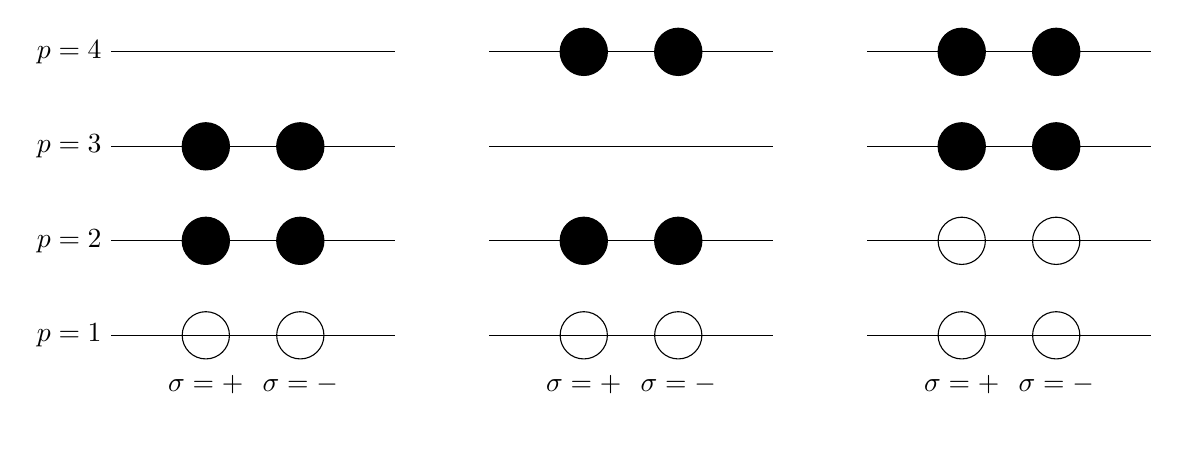
\begin{tikzpicture}[scale=1.2]
    \begin{scope}
      \foreach \i in {1,...,4}
      {
        \draw (-1,\i-1) node[anchor=east] {$p = \i$} --(2,\i-1);
      }
      \draw (0,0) node[anchor=north,inner sep=.5cm] {$\sigma=+$} circle (0.25cm); 
      \draw (1,0) node[anchor=north,inner sep=.5cm] {$\sigma=-$} circle (0.25cm);
      \filldraw (0,1) circle (0.25cm); 
      \filldraw (1,1) circle (0.25cm);
      \filldraw (0,2) circle (0.25cm); 
      \filldraw (1,2) circle (0.25cm);
    \end{scope}
    \begin{scope}[xshift=4cm]
      \foreach \i in {1,...,4}
      {
        \draw (-1,\i-1) --(2,\i-1);
      }
      \draw (0,0) node[anchor=north,inner sep=.5cm] {$\sigma=+$} circle (0.25cm); 
      \draw (1,0) node[anchor=north,inner sep=.5cm] {$\sigma=-$} circle (0.25cm);
      \filldraw (0,1) circle (0.25cm); 
      \filldraw (1,1) circle (0.25cm);
      \filldraw (0,3) circle (0.25cm); 
      \filldraw (1,3) circle (0.25cm);
    \end{scope}
    \begin{scope}[xshift=8cm]
      \foreach \i in {1,...,4}
      {
        \draw (-1,\i-1) --(2,\i-1);
      }
      \draw (0,0) node[anchor=north,inner sep=.5cm] {$\sigma=+$} circle (0.25cm); 
      \draw (1,0) node[anchor=north,inner sep=.5cm] {$\sigma=-$} circle (0.25cm);
      \draw (0,1) circle (0.25cm); 
      \draw (1,1) circle (0.25cm);
      \filldraw (0,2) circle (0.25cm); 
      \filldraw (1,2) circle (0.25cm);
      \filldraw (0,3) circle (0.25cm); 
      \filldraw (1,3) circle (0.25cm);
    \end{scope}
  \end{tikzpicture}
\end{center}
\caption{Above all basis states of our pair interaction system are presented schematically with $P=2$ as the number of pairs and $S_z=0$ are the total spin. The solid dots indicate occupied states, while the empty dots indicate unoccupied states (holes). The reference state $|\Phi\rangle$ is represented in the upper left corner. This is all possible states since the excusion principle does not allow two particles with same spin to stay at the same level. For further description, see the text.\label{fig:schematic}}
\end{figure*}
We have a pairwise system, where each particle needs to have a partner in the same level with opposite spin. From figure (\ref{fig:schematic}) one can observe that the dimension of the subspace for $M=4$ is $3+2+1=6$, which is the number of possible states. We can easily imagine that for $M=2$ we would get 1 state, with $M=5$ we would get $4+3+2+1=10$ states and so on. Thus the dimension of the subspace for an arbitrary $M$ is given by the arithmetic series
\begin{equation}
n_M=\sum_{m=1}^{M-1}(M-m).
\end{equation}

\subsection*{1G}
With $P=0$ we do not have any pairs, so the only state consists of unoccupied states (but not holes, since they are not surrounded by particles). I do not find it necessary to draw this, since it just will be a state without particles.

\subsection*{1H}
\begin{equation*}
\hat{H}=\hat{H_0}+\hat{V}
\end{equation*}
We use equation (\ref{eq:H0_init}) and (\ref{eq:V_init}), and get
\begin{align*}
\hat{V}&=-\frac{1}{2}g\sum_{pq}c_{p+}^{\dagger}c_{p-}^{\dagger}c_{q-}c_{q+}\notag\\
&=-\frac{1}{2}g\sum_{p}^Mc_{p+}^{\dagger}c_{p-}^{\dagger}\sum_q^Mc_{q-}c_{q+}\notag\\
&=-\frac{1}{2}g\bigg(\sum_{p=1}^4\hat{P}_p^{\dagger}\bigg)\bigg(\sum_{q=1}^4\hat{P}_q\bigg)
\end{align*}
Similarly we get
\begin{align*}
\hat{H_0}&=\sum_{p\sigma}\varepsilon_pc_{p\sigma}^{\dagger}c_{p\sigma}\notag\\
&=\sum_p(p-1)\sum_{\sigma}c_{p\sigma}^{\dagger}c_{p\sigma}\notag\\
&=\sum_p(p-1)\hat{n}_p.
\end{align*}
Thus we end up with
\begin{equation}
\hat{H}=\sum_p(p-1)\hat{n}_p-\frac{1}{2}g\bigg(\sum_{p=1}^4\hat{P}_p^{\dagger}\bigg)\bigg(\sum_{q=1}^4\hat{P}_q\bigg)
\end{equation}

\newpage
\section{Configuration-Interaction (CI)}
\subsection*{2A}
\begin{align}
\sum_s\hat{P}_s|p\bar{p}q\bar{q}\rangle=&\sum_s\hat{P}_s\hat{P}_p^{\dagger}\hat{P}_q^{\dagger}|-\rangle
\label{eq:2Aa}
\end{align}
We use the result from exercise 1D (equation (\ref{eq:ex1d})) twice, and get
\begin{align*}
\hat{P}_s\hat{P}_p^{\dagger}\hat{P}_q^{\dagger}
=&\hat{P}_p^{\dagger}\hat{P}_s\hat{P}_q^{\dagger}+\delta_{sp}(1-\hat{n}_p)\hat{P}_q^{\dagger}\notag\\
=&\hat{P}_p^{\dagger}\hat{P}_q^{\dagger}\hat{P}_s+\hat{P}_p^{\dagger}\delta_{sq}(1-\hat{n}_q)+\delta_{sp}(1-\hat{n}_p)\hat{P}_q^{\dagger}
\end{align*}
Then insert back into equation (\ref{eq:2Aa}):
\begin{align*}
&\sum_s(\hat{P}_p^{\dagger}\hat{P}_q^{\dagger}\hat{P}_s+\hat{P}_p^{\dagger}\delta_{sq}(1-\hat{n}_q)+\delta_{sp}(1-\hat{n}_p)\hat{P}_q^{\dagger})|-\rangle\notag\\
&=\sum_s(\hat{P}_p^{\dagger}\delta_{sq}(1-\hat{n}_q)+\delta_{sp}(1-\hat{n}_p)\hat{P}_q^{\dagger})|-\rangle\notag\\
&=\sum_s(\delta_{sq}\hat{P}_p^{\dagger}-\delta_{sq}\hat{P}_p^{\dagger}\hat{n}_q+\delta_{sp}\hat{P}_q^{\dagger}-\delta_{sp}\hat{n}_p\hat{P}_q^{\dagger})|-\rangle\notag\\
&=\sum_s(\delta_{sp}\hat{P}_p^{\dagger}+\delta_{sq}\hat{P}_q^{\dagger})|-\rangle\notag\\
&=(\hat{P}_p^{\dagger}+\hat{P}_q^{\dagger})|-\rangle\notag\\
&=|p\bar{p}\rangle+|q\bar{q}\rangle
\end{align*}
Firstly the first term vanishes, since an annihilation operator acts on the vacuum. Also when $\hat{n}_p$ acts on vacuum the term dies, and since this operator is hermitian, it can always be moved to the vacuum. Further we will find the Hamiltonian matrix
\begin{equation*}
\langle p'\bar{p}'q'\bar{q}|\hat{H}|p\bar{p}q\bar{q}\rangle=\langle p'\bar{p}'q'\bar{q}|\hat{H}_0|p\bar{p}q\bar{q}\rangle+\langle p'\bar{p}'q'\bar{q}|\hat{V}|p\bar{p}q\bar{q}\rangle
\end{equation*}
I will start with the first one:
\begin{equation*}
\hat{H}_0|p\bar{p}q\bar{q}\rangle = \sum_{r\sigma}\epsilon_rc_{r\sigma}^{\dagger}c_{r\sigma}c_{p+}^{\dagger}c_{p-}^{\dagger}c_{q+}^{\dagger}c_{q-}^{\dagger}|-\rangle
\end{equation*}
Wick's theorem is used to calculate this, and since it requires normal ordering, the vacuum state will kill all strings including an annihilation operator. In this case we therefore get four terms which come from single contraction. We will get delta functions, which only contribute when both indexes are equal, so for instance if we get $\delta_{rp}$ we need to set $r=p$ since $r$ runs over all possible states.
\begin{align}
\hat{H}_0|p\bar{p}q\bar{q}\rangle 
&= \sum_{r\sigma}\epsilon_r\{c_{r\sigma}^{\dagger}c_{p+}^{\dagger}c_{p-}^{\dagger}c_{q+}^{\dagger}c_{q-}^{\dagger}c_{r\sigma}\}|-\rangle\notag\\
&\mathrel{\phantom{=}}+\sum_{r\sigma}\epsilon_r\delta_{r\sigma p+}c_{r\sigma}^{\dagger}c_{p-}^{\dagger}c_{q+}^{\dagger}c_{q-}^{\dagger}|-\rangle\notag\\
&\mathrel{\phantom{=}}-\sum_{r\sigma}\epsilon_r\delta_{r\sigma p-}c_{r\sigma}^{\dagger}c_{p+}^{\dagger}c_{q+}^{\dagger}c_{q-}^{\dagger}|-\rangle\notag\\
&\mathrel{\phantom{=}}+\sum_{r\sigma}\epsilon_r\delta_{r\sigma q+}c_{r\sigma}^{\dagger}c_{p+}^{\dagger}c_{p-}^{\dagger}c_{q-}^{\dagger}|-\rangle\notag\\
&\mathrel{\phantom{=}}-\sum_{r\sigma}\epsilon_r\delta_{r\sigma q-}c_{r\sigma}^{\dagger}c_{p+}^{\dagger}c_{p-}^{\dagger}c_{q+}^{\dagger}|-\rangle\notag\\
&=(\epsilon_pc_{p+}^{\dagger}c_{p-}^{\dagger}c_{q+}^{\dagger}c_{q-}^{\dagger}-\epsilon_pc_{p-}^{\dagger}c_{p+}^{\dagger}c_{q+}^{\dagger}c_{q-}^{\dagger}\notag\\
&\mathrel{\phantom{=}}+\epsilon_qc_{q+}^{\dagger}c_{p+}^{\dagger}c_{p-}^{\dagger}c_{q-}^{\dagger}-\epsilon_qc_{q-}^{\dagger}c_{p+}^{\dagger}c_{p-}^{\dagger}c_{q+}^{\dagger})|-\rangle\notag\\
&=(\epsilon_pc_{p+}^{\dagger}c_{p-}^{\dagger}c_{q+}^{\dagger}c_{q-}^{\dagger}+\epsilon_pc_{p+}^{\dagger}c_{p-}^{\dagger}c_{q+}^{\dagger}c_{q-}^{\dagger}\notag\\
&\mathrel{\phantom{=}}+\epsilon_qc_{p+}^{\dagger}c_{p-}^{\dagger}c_{q+}^{\dagger}c_{q-}^{\dagger}+\epsilon_qc_{p+}^{\dagger}c_{p-}^{\dagger}c_{q+}^{\dagger}c_{q-}^{\dagger})|-\rangle\notag\\
&=2(\epsilon_p+\epsilon_q)(\hat{P}_p^{\dagger}\hat{P}_p^{\dagger})|-\rangle\notag\\
&=-2(2-p-q)|p\bar{p}q\bar{q}\rangle
\end{align} 
where $\xi=1$ is assumed. We then get
\begin{equation}
\langle p'\bar{p}'q'\bar{q}'|\hat{H}_0|p\bar{p}q\bar{q}\rangle=-2(2-p-q)\langle p'\bar{p}'q'\bar{q}'|p\bar{p}q\bar{q}\rangle
\end{equation}
So we still need to calculate the braket (puh)
\begin{equation*}
\langle p'\bar{p}'q'\bar{q}'|p\bar{p}q\bar{q}\rangle=\langle-|\hat{P}_{p'}\hat{P}_{q'}\hat{P}_p^{\dagger}\hat{P}_q^{\dagger}|-\rangle
\end{equation*}
Again we will try to move the annihilation operator all the way to the right, such that it acts on the vacuum. The result from exercise 1D will be applied several times.
\begin{align*}
\hat{P}_{p'}\hat{P}_{q'}\hat{P}_p^{\dagger}\hat{P}_q^{\dagger}&=\hat{P}_{p'}\hat{P}_p^{\dagger}\hat{P}_{q'}\hat{P}_q^{\dagger}+\delta_{q'p}\hat{P}_{p'}(1-\hat{n}_p)\hat{P}_q^{\dagger}\\
&=\hat{P}_{p'}\hat{P}_p^{\dagger}\hat{P}_{q'}\hat{P}_q^{\dagger}+\delta_{q'p}\hat{P}_{p'}\hat{P}_q^{\dagger}+\delta_{q'p}\hat{P}_{p'}\hat{n}_p\hat{P}_q^{\dagger}
\end{align*}
Since $\hat{n}_p$ is hermitian, we can move it to the right in the last term, and the term will vanish when it acts on the vacuum state. From now on I will stop commenting that annihilators are killed by the vacuum. The second term becomes
\begin{align*}
\delta_{q'p}\hat{P}_{p'}\hat{P}_q^{\dagger}&=\delta_{q'p}\hat{P}_q^{\dagger}\hat{P}_{p'}+\delta_{q'p}\delta_{p'q}+\delta_{q'p}\delta_{p'q}\hat{n}_q\\
&=\delta_{q'p}\delta_{p'q}
\end{align*}
while the first term is slightly more complicated. We need to switch the two latter operators to get the annihilation operator acting in vacuum:
\begin{align*}
\hat{P}_{p'}\hat{P}_p^{\dagger}\hat{P}_{q'}\hat{P}_q^{\dagger}&=\hat{P}_{p'}\hat{P}_p^{\dagger}\hat{P}_{q}^{\dagger}\hat{P}_{q'}+\delta_{q'q}\hat{P}_{p'}\hat{P}_p^{\dagger}(1-\hat{n}_q)\\
&=\delta_{q'q}\hat{P}_{p'}\hat{P}_p^{\dagger}\\
&=\delta_{q'q}\delta_{p'p}-\delta_{q'q}\delta_{p'p}\hat{n}_q+\delta_{q'q}\hat{P}_p^{\dagger}\hat{P}_{p'}\\
&=\delta_{q'q}\delta_{p'p}
\end{align*}
So we obtain
\begin{equation}
\langle p'\bar{p}'q'\bar{q}'|p\bar{p}q\bar{q}\rangle=\delta_{q'p}\delta_{p'q}+\delta_{q'q}\delta_{p'p}
\end{equation}
and 
\begin{equation}
\langle p'\bar{p}'q'\bar{q}'|\hat{H}_0|p\bar{p}q\bar{q}\rangle=-2(2-p-q)(\delta_{q'p}\delta_{p'q}+\delta_{q'q}\delta_{p'p}).
\end{equation}
One term done, one to go. Fortunately the potential term is much easier to calculate:
\begin{align*}
\langle p'\bar{p}'q'\bar{q}|\hat{V}|p\bar{p}q\bar{q}\rangle=-\frac{1}{2}g\langle p'\bar{p}'q'\bar{q}|(\sum_r\hat{P}_r^{\dagger})(\sum_s\hat{P}_s)|p\bar{p}q\bar{q}\rangle
\end{align*}
In the beginning of this exercise we proved that $\sum_s\hat{P}_s|p\bar{p}q\bar{q}\rangle=|p\bar{p}\rangle+|q\bar{q}\rangle$. Similarly one can prove the corresponding hermitian conjugate
\begin{equation}
\langle p'\bar{p}'q'\bar{q}'|\sum_r\hat{P}_r^{\dagger}=\langle p'\bar{p}'|+\langle q'\bar{q}'|
\end{equation}
With this in mind, we can rewrite the potential braket into four small brakets
\begin{equation}
\langle p'\bar{p}'q'\bar{q}|\hat{V}|p\bar{p}q\bar{q}\rangle=-\frac{1}{2}g(\langle p'\bar{p}'|p\bar{p}\rangle+\langle p'\bar{p}'|q\bar{q}\rangle+\langle q'\bar{q}'|p\bar{p}\rangle+\langle q'\bar{q}'|q\bar{q}\rangle)
\end{equation}
where the former is
\begin{equation}
\langle p'\bar{p}'|p\bar{p}\rangle=\langle -|\hat{P}_{p'}\hat{P}_p^{\dagger}|-\rangle=\langle -|\hat{P}_{p}^{\dagger}\hat{P}_{p'}+\delta_{p'p}(1-\hat{n}_p)|-\rangle=\delta_{p'p}
\end{equation}
and similar for the other three. We can finally write out the matrix element expression
\begin{equation}
\langle p'\bar{p}'q'\bar{q}|\hat{H}|p\bar{p}q\bar{q}\rangle=-2(2-p-q)(\delta_{q'p}\delta_{p'q}+\delta_{q'q}\delta_{p'p})-\frac{1}{2}g(\delta_{p'p}+\delta_{p'q}+\delta_{q'p}+\delta_{q'q})
\end{equation}
Observe that the first term from $\hat{H}_0$ will never contribute since Pauli's exclusion principle restricts $q>p$ (and $q'>p'$). $\hat{H}_0$ will therefore only make contributions on the diagonal when we form a matrix based on Full Configuration-Interactions (as expected). It is also worth to notice that there will not be any contribution if all the indexes are different.

\subsection*{2B}
In our case we get a matrix on the form
\begin{equation*}
\begin{pmatrix} 
H_{12}^{12}&H_{12}^{13}&H_{12}^{14}&H_{12}^{23}&H_{12}^{24}&H_{12}^{34}\\
H_{13}^{12}&H_{13}^{13}&H_{13}^{14}&H_{13}^{23}&H_{13}^{24}&H_{13}^{34}\\
H_{14}^{12}&H_{14}^{13}&H_{14}^{14}&H_{14}^{23}&H_{14}^{24}&H_{14}^{34}\\
H_{23}^{12}&H_{23}^{13}&H_{23}^{14}&H_{23}^{23}&H_{23}^{24}&H_{23}^{34}\\
H_{24}^{12}&H_{24}^{13}&H_{24}^{14}&H_{24}^{23}&H_{24}^{24}&H_{24}^{34}\\
H_{34}^{12}&H_{34}^{13}&H_{34}^{14}&H_{34}^{23}&H_{34}^{24}&H_{34}^{34} \end{pmatrix}
\end{equation*}
where 
\begin{equation*}
H_{12}^{34}=\langle 12|\hat{H}|34\rangle=2(2-3-4)(0+0)-\frac{1}{2}g(0+0+0+0)=0
\end{equation*}
etc.. Calculate all elements, and get
\begin{equation}
\langle p'\bar{p}'q'\bar{q}|\hat{H}|p\bar{p}q\bar{q}\rangle=\begin{pmatrix} 
2-g&-1/2g&-1/2g&-1/2g&-1/2g&0\\
-1/2g&4-g&-1/2g&-1/2g&0&-1/2g\\
-1/2g&-1/2g&6-g&0&-1/2g&-1/2g\\
-1/2g&-1/2g&0&6-g&-1/2g&-1/2g\\
-1/2g&0&-1/2g&-1/2g&8-g&-1/2g\\
0&-1/2g&-1/2g&-1/2g&-1/2g&10-g \end{pmatrix}.
\label{eq:FCI_matrix}
\end{equation}
The eigenvalues of the Hamiltonian are the diagonal elements after diagonalization, and we find them using the numpy package in Python (see Appendix A). The eigenvalues as a function of $g$ are plotted in figure (\ref{fig:eigenvalues_FCI}).
\begin{figure}[h]
\centering
\includegraphics[width=100mm]{eigenvalues_FCI.png}
\caption{Above the (exact) FCI energies are presented as a function of $g$, where $g\in[-1,1]$. The reference energy is highlighted with a thick line. See text for further description. \label{fig:eigenvalues_FCI}}
\end{figure}
We can only spot 5 eigenvalue lines, even though we know it should be 6 and the legend tells us there is 6 eigenvalues. The reason is obvious, eigenvalue 3 is hidden behind eigenvalue 4 since they are identical. We have a double degeneracy, i.e, the energy of state 3 and 4 are the same. Further, we have studied the probability of finding a system in the unperturbed ground state. Since the script in Appendix A gives the eigenvectors, this task was solved numerically by extending that script. In figure (\ref{fig:prob_FCI}) the true probability is plotted as function of $g$.

\begin{figure}[H]
\centering
\includegraphics[width=100mm]{probability_FCI.png}
\caption{The exact probability (from FCI) of finding the system in the unperturbed groundstate. $g$ spans from -1 to 1. \label{fig:prob_FCI}}
\end{figure}

As we can see, the probability is 0 at $g=0$ and decreasing as $g$ increases. This is reasonable because all the system is unperturbed when $g$, so we are guaranteed to find the system in the unperturbed ground state. See Appendix B for the actual program code. 

\subsection*{2C}
The single excited determinants ($|\Phi_i^a\rangle$) will not contribute to the exact eigenfunction since we require $a=b$, i.e two particles with opposite spin shall always be at the same level. We will work with Configuration-Interaction Doubles (CID), but have in mind that it is the same as Configuration-Interaction Singles-Doubles (CISD). In general the doubly excited determinants can be written
\begin{equation}
|\Phi_{ij}^{ab}\rangle=c_a^{\dagger}c_b^{\dagger}c_ic_j|\Phi\rangle
\end{equation}
In our case the first unoccupied index $a$ has positive spin, while the second has negative spin. Since they both will be at the same level, the second index is denoted with a bar, which implies negative spin. Similarly the second occupied index has negative spin, so we have
\begin{equation}
|\Phi_{i\bar{i}}^{a\bar{a}}\rangle=c_{a+}^{\dagger}c_{a-}^{\dagger}c_{i+}c_{i-}|\Phi\rangle=\hat{P}_a^{\dagger}\hat{P}_i|\Phi\rangle
\end{equation}
In our case the CID matrix will be a 5x5 matrix where the last column and the last row is dropped:
\begin{equation}
M_{CID}=\begin{pmatrix} 
2-g&-1/2g&-1/2g&-1/2g&-1/2g\\
-1/2g&4-g&-1/2g&-1/2g&0&\\
-1/2g&-1/2g&6-g&0&-1/2g\\
-1/2g&-1/2g&0&6-g&-1/2g\\
-1/2g&0&-1/2g&-1/2g&8-g\end{pmatrix}.
\end{equation}
and we are curious if we get a significant change in the groundstate energy. In figure (\ref{fig:groundstate_comparison}) the ground-state energy from FCI is plotted together with the CID ground-state energy. This plot was made by the code in Appendix C.

\begin{figure}[H]
\centering
\includegraphics[width=100mm]{groundstate_comparison.png}
\caption{The FCI and CID ground-state (GS) energy as functions of $g$ where $g$ runs from -1 to 1.  \label{fig:groundstate_comparison}}
\end{figure}

Considering that we dropped 11 matrix elements, the approximation looks satisfying. Actually it is hard to see any difference at first glance, but if we look carefully, we can spot small errors when the absolute value of $g$ is increasing. Furthermore the CID probability of finding the system in the unperturbed groundstate can be found in figure (\ref{fig:prob_CID}), and we observe that it is quite similar to that we had for FCI, which is a good sign. The script used to plot this is a extension of the script found in Appendix B. 

\begin{figure}[H]
\centering
\includegraphics[width=100mm]{probability_CID.png}
\caption{The CID probability of finding the system in the unperturbed groundstate. $g$ spans from -1 to 1.\label{fig:prob_CID}}
\end{figure}

\subsection*{2D}
The non-degenerate Rayleigh-Schrodinger Perturbation Theory (RSPT) energy is given by
\begin{equation}
E^{(n)}=\langle \Phi|\hat{V}|\Psi^{(n-1)}\rangle
\end{equation}
with
\begin{equation}
|\Psi^{(n)}\rangle=\hat{R}\bigg[\hat{V}|\Phi^{(n-1)}\rangle-\sum_{j=1}^{n-1}|\Psi^{(j)}\rangle\bigg].
\end{equation}
The first order energy correction becomes
\begin{equation*}
E^{(1)}=\langle\Phi|\hat{V}|\Psi^{(0)}\rangle=\langle\Phi|\hat{V}|\Phi\rangle.
\end{equation*}
We also calculate $|\Psi^{(1)}\rangle$, which we will need for higher order energy expressions. 
\begin{equation*}
|\Psi^{(1)}\rangle=\hat{R}\bigg[\hat{V}|\Psi^{(0)}\rangle-\sum_{j=1}^{0}E^{(1-j)}|\Psi^{(j)}\rangle\bigg]=\hat{R}\hat{V}|\Phi\rangle
\end{equation*}
We then obtain the following for the second order correction:
\begin{equation*}
E^{(2)}=\langle\Phi|\hat{V}|\Psi^{(1)}\rangle=\langle\Phi|\hat{V}\hat{R}\hat{V}|\Phi\rangle
\end{equation*}
and
\begin{equation*}
|\Psi^{(2)}\rangle=\hat{R}\bigg[\hat{V}\hat{R}\hat{V}|\Phi\rangle-E^{(1)}|\Psi^{(1)}\rangle\bigg]=\hat{R}\bigg[\hat{V}-\langle\Phi|\hat{V}|\Phi\rangle\bigg]\hat{R}\hat{V}|\Phi\rangle.
\end{equation*}
Finally we can compute the third order correction energy:
\begin{equation*}
E^{(3)}=\langle\Phi|\hat{V}\hat{R}\hat{V}\hat{R}\hat{V}|\Phi\rangle-\langle\Phi|\hat{V}|\Phi\rangle\langle\Phi|\hat{V}\hat{R}\hat{R}\hat{V}|\Phi\rangle
\end{equation*}
We can see that the first term follows a certain pattern for increasing order corrections, and is considered as the leading term. The second term is smaller, and for rough estimates it is sometimes omitted. Further we can insert $\hat{R}$ expression:
\begin{equation}
\hat{R}=\sum_{j,j\neq k}\frac{1}{\epsilon_k-\epsilon_j}|\Phi_j\rangle\langle\Phi_j|
\end{equation}
such that $\hat{V}$ is the only operator to take care of:
\begin{align}
E_k^{(1)}&=\langle\Phi_k|\hat{V}|\Phi_k\rangle\\
E_k^{(2)}&=\sum_{j,j\neq k}\frac{|\langle\Phi_k|\hat{V}|\Phi_j\rangle|^2}{\epsilon_k-\epsilon_j}\\
E_k^{(3)}&=\sum_{j,j\neq k}\sum_{j',j'\neq k}\frac{\langle\Phi_k|\hat{V}|\Phi_j\rangle\langle\Phi_j|\hat{V}|\Phi_{j'}\rangle\langle\Phi_{j'}|\hat{V}|\Phi_k\rangle}{(\epsilon_k-\epsilon_j)(\epsilon_k-\epsilon_{j'})}\notag\\
&\mathrel{\phantom{=}}-\sum_{j,j\neq k}\frac{\langle\Phi_k|\hat{V}|\Phi_k\rangle\langle\Phi_k|\hat{V}|\Phi_{j}\rangle\langle\Phi_j|\hat{V}|\Phi_k\rangle}{(\epsilon_k-\epsilon_j)(\epsilon_k-\epsilon_j)}
\end{align}

\subsection*{2E}
We are now going to compute the ground state energy to third order in Rayleigh-Schrodinger perturbation theory
\begin{equation}
E_{RSPT3}=E^{(0)}+gE^{(1)}+g^2E^{(2)}+g^3E^{(3)}.
\end{equation}
where $E^{(0)}=\langle\Phi|\hat{H}_0|\Phi\rangle=2$ is the ground energy and the other energies are expressed in the previous exercise ($k$ is set to be 0). There are two way to compute this: We could either use second quantization and many-body perturbation theory (MBPT) or we could use basic PT on matrix form. Since the latter already is derived, we better use that method. 

Set $k=0$ for the other terms, and use the matrix in equation (\ref{eq:FCI_matrix}) to find the products. We obtain
\begin{align*}
E^{(1)}=-g
\end{align*}
\begin{align*}
E^{(2)}&=\frac{1}{\epsilon_0-\epsilon_1}\Big(\frac{1}{2}g\Big)^2+\frac{1}{\epsilon_0-\epsilon_2}\Big(\frac{1}{2}g\Big)^2+\frac{1}{\epsilon_0-\epsilon_3}\Big(\frac{1}{2}g\Big)^2+\frac{1}{\epsilon_0-\epsilon_4}\Big(\frac{1}{2}g\Big)^2\\
&=-\Big(1+\frac{1}{2}+\frac{1}{3}+\frac{1}{4}\Big)\cdot\frac{1}{4}g^2=-\frac{25}{48}g^2
\end{align*}
The last term, $E^{(3)}$, is far the most complicated, and it is easy to make mistakes. We work out the first and the last part separately:
\begin{align*}
&\sum_{j,j\neq k}\sum_{j',j'\neq k}\frac{\langle\Phi_k|\hat{V}|\Phi_j\rangle\langle\Phi_j|\hat{V}|\Phi_{j'}\rangle\langle\Phi_{j'}|\hat{V}|\Phi_k\rangle}{(\epsilon_k-\epsilon_j)(\epsilon_k-\epsilon_{j'})}\\
&=-\Big(\frac{1}{4}+2\cdot\frac{1}{16}+2\cdot\frac{1}{24}+2\cdot\frac{1}{48}+2\cdot\frac{1}{96}+\frac{1}{36}+\frac{1}{128}\Big)g^3\\
&=-\frac{641}{1152}g^3
\end{align*}
Among the 20 terms in the sum, 9 is zero, and we get a relatively nasty fraction. For the second part we get
\begin{align*}
&\sum_{j,j\neq k}\frac{\langle\Phi_k|\hat{V}|\Phi_k\rangle\langle\Phi_k|\hat{V}|\Phi_{j}\rangle\langle\Phi_j|\hat{V}|\Phi_k\rangle}{(\epsilon_k-\epsilon_j)(\epsilon_k-\epsilon_j)}\\
&=-\frac{1}{4}\Big(1+\frac{1}{4}+\frac{1}{9}+\frac{1}{16}\Big)\\
&=-\frac{410}{1152}g^3
\end{align*}
In total we get 
\begin{equation*}
E^{(3)}=-\frac{641}{1152}g^3+\frac{410}{1152}g^3=-\frac{231}{1152}g^3
\end{equation*}
and our RSPT3 approximation becomes
\begin{equation}
E_{RSPT3}(g)=2 - g^2 + (25/48)*g**4 - (231/1152)*g**6
\end{equation}

\newpage
\section{Coupled-Cluster (CC)}
\subsection*{3A}
The general CCD wavefunction is as following
\begin{equation}
|\Psi_{CID}\rangle=\exp{(\hat{T})}|\Phi\rangle=(1+\hat{T}+\frac{1}{2}\hat{T}^2)|\Phi\rangle
\end{equation}
Because our system contains of only four particles, higher order terms do not appear. 

\subsection*{3B}
\begin{align}
|\Psi_{CID}\rangle&=(1+\hat{C}_2)|\phi\rangle=(1+\hat{T})|\Phi\rangle\\
|\Psi_{CCD}\rangle&=|\Psi_{CID}\rangle+(1/2\hat{T}^2)|\Phi\rangle
\end{align}

\subsection*{3C}
\begin{equation*}
\langle \Phi|\hat{H}(1+\hat{T})|\Phi\rangle=\langle \Phi|\hat{H}|\Phi\rangle+\langle \Phi|\hat{H}\hat{T}|\Phi\rangle
\end{equation*}
The first term is already calculated, and we found it to be $(2(\epsilon_p+\epsilon_q)-g)(\delta_{p'p}+\delta_{p'q}+\delta_{q'p}+\delta_{q'q})$. In this case we deal with the reference wave function, such that $p'=p$ and $q'=q$. We then obtain
\begin{equation*}
\langle \Phi|\hat{H}|\Phi\rangle=2\epsilon_p+2\epsilon_q-g
\end{equation*}

Furthermore we work out the second term. Recall that $a$ is an unoccupied index, $i$ is occupied and $p, , rq$ and $s$ are arbitrary indexes. Because of $\hat{H}$ we can immediately see that the term again can be split up in two new terms:
\begin{align*}
\langle\Phi|\hat{H}|\Phi\rangle&=\langle p'\bar{p}'q'\bar{q}'|(\sum_r(r-1)\hat{n}_r)(\sum_{ia}t_i^a\hat{P}_a^{\dagger}\hat{P}_i)|p\bar{p}q\bar{q}\rangle\notag\\
&\mathrel{\phantom{=}}+\langle p'\bar{p}'q'\bar{q}'|-\frac{1}{2}g(\sum_{r}\hat{P}_r^{\dagger})(\sum_s\hat{P}_s)(\sum_{ia}t_i^a\hat{P}_a^{\dagger}\hat{P}_i)|p\bar{p}q\bar{q}\rangle
\end{align*}
We first examine the first of these terms:
\begin{align*}
\langle p'\bar{p}'q'\bar{q}'|(\sum_r(r-1)\hat{n}_r)(\sum_{ia}t_i^a\hat{P}_a^{\dagger}\hat{P}_i)|p\bar{p}q\bar{q}\rangle=\sum_{ria}\epsilon_r\langle-|\hat{P}_{p}\hat{P}_p^{\dagger}(\sum_{\sigma}c_{r\sigma}^{\dagger}c_{r\sigma})\hat{P}_a^{\dagger}\hat{P}_i|-\rangle
\end{align*}
We could calculate this, but instead I will argue why it becomes zero. The rightmost operator is an annihilation operator, which means that it never will be contracted in a non-zero term. If we use Wick's theorem on the operators, we then will have an annihilation operator in every term, and since we need to leave them on normal order, we will always have an annihilation operator acting on the vacuum which is zero by definition. 

Further we need to calculate the second term. 
\begin{align*}
&\langle p'\bar{p}'q'\bar{q}'|-\frac{1}{2}g(\sum_{r}\hat{P}_r^{\dagger})(\sum_s\hat{P}_s)(\sum_{ia}t_i^a\hat{P}_a^{\dagger}\hat{P}_i)|p\bar{p}q\bar{q}\rangle\notag\\
=&-\frac{1}{2}g\sum_{rsia}t_i^a\langle-|\hat{P}_{p'}\hat{P}_{q'}\hat{P}_r^{\dagger}\hat{P}_s\hat{P}_a^{\dagger}\hat{P}_i\hat{P}_p^{\dagger}\hat{P}_q^{\dagger}|-\rangle
\end{align*}
We will now use Wick's theorem on the operators. On the same basis as for the first term, only terms without annihilation operators will contribute. There are several possible fully contracted terms, but we need to keep in mind that if an arbitrary operator has contracted to say an occupied index, it can only be contracted to occupied indexes. The fully contracted term is therefore 
\begin{align*}
\{\hat{P}_{p'}\hat{P}_{q'}\hat{P}_r^{\dagger}\hat{P}_s\hat{P}_a^{\dagger}\hat{P}_i\hat{P}_p^{\dagger}\hat{P}_q^{\dagger}\}_{fc}
&=\wick{\c2 c_{p'-}\c1 c_{p'+}\c6 c_{q'-}\c5 c_{q'+}\c1 c_{r+}^{\dagger}\c2 c_{r-}^{\dagger}\c4 c_{s-}\c3 c_{s+}\c5 c_{a+}^{\dagger}\c6 c_{a-}^{\dagger}\c2 c_{i-}\c1 c_{i+}\c1 c_{p+}^{\dagger}\c2 c_{p-}^{\dagger}\c3 c_{q+}^{\dagger}\c4 c_{q-}^{\dagger}}\\
&=\delta_{p'r}\delta_{p'r}\delta_{q'a}\delta_{q'a}\delta_{sq}\delta_{sq}\delta_{ip}\delta_{ip}
\end{align*}
Again the sum runs over all possible indexes, i.e, at one point we will have $p=i$, $q'=a$, $s=q$ and $r=p'$, and we get contribution. After some argumentation, we obtain
\begin{equation}
E_{CCD}=2\epsilon_1+2\epsilon_2-g-\frac{1}{2}g\sum_{ia}t_i^a
\end{equation}

\subsection*{3D}
The normal ordered Fock operator is given by 
\begin{equation}
\{\hat{F}\}=\hat{H}_0^{(1qp)}+\hat{V}^{(1qp)}
\end{equation}
where $(1qp)$ indicates one quasi particle. If we apply Wick's theorem on $\hat{H}_0$, we get
\begin{align*}
\hat{H}_0&=\sum_{p\sigma}\epsilon_{p\sigma}^{\dagger}c_{p\sigma}\notag\\
&=\sum_{p\sigma}\epsilon_{p}\{c_{p\sigma}^{\dagger}c_{p\sigma}\}+\sum_{p\sigma}\epsilon_p\wick{\c c_{p\sigma}^{\dagger}\c c_{p\sigma}}\notag\\
&=\sum_{i\sigma}\epsilon_{i}\{c_{i\sigma}^{\dagger}c_{i\sigma}\}+\sum_{i\sigma}\epsilon_i\wick{\c c_{i\sigma}^{\dagger}\c c_{i\sigma}}+\sum_{a\sigma}\epsilon_{a}\{c_{a\sigma}^{\dagger}c_{a\sigma}\}+\sum_{a\sigma}\epsilon_a\wick{\c c_{a\sigma}^{\dagger}\c c_{a\sigma}}\notag\\
&=\sum_{i\sigma}\epsilon_{i}\{c_{i\sigma}^{\dagger}c_{i\sigma}\}+\sum_i\epsilon_i+\sum_{a\sigma}\epsilon_{a}\{c_{a\sigma}^{\dagger}c_{a\sigma}\}\notag\\
&=\sum_{p\sigma}\epsilon_{p}\{c_{p\sigma}^{\dagger}c_{p\sigma}\}+\sum_i\epsilon_i
\end{align*} 
where the first term corresponds to one quasi particle and the second corresponds to zero quasi particles. For the potential operator I will only calculate the $(1qp)$ part, which is the terms we get from Wick's theorem with one contraction. 
\begin{align*}
\hat{V}^{(1qp)}&=-\frac{1}{2}g\sum_{pq}(\wick{\c1 c_{p+}^{\dagger}c_{p-}^{\dagger}c_{q-}\c1 c_{q+}+c_{p+}^{\dagger}\c2 c_{p-}^{\dagger}\c2 c_{q-}c_{q+}})\notag\\
&=-\frac{1}{2}g\sum_{pq}(\wick{\c1 c_{i+}^{\dagger}c_{i-}^{\dagger}c_{j-}\c1 c_{j+}+c_{i+}^{\dagger}\c2 c_{i-}^{\dagger}\c2 c_{j-}c_{j+}})\notag\\
&=-\frac{1}{2}g\sum_{ij}(\delta_{ij}c_{i-}^{\dagger}c_{j-}+\delta_{ij}c_{i+}^{\dagger}c_{j+})\notag\\
&=-\frac{1}{2}g\sum_{i\sigma}c_{i\sigma}^{\dagger}c_{i\sigma}
\end{align*}
where we observed that all the unoccupied operators became zero since $c_{p}^{\dagger}c_{q}=b_{p}^{\dagger}b_{q}=0$. We then use the definition of the Fock operator:
\begin{align}
\hat{F}_N&=\hat{H}_0^{(1qp)}+\hat{V}^{(1qp)}\notag\\
&=\sum_{i\sigma}\epsilon_{i}\{c_{i\sigma}^{\dagger}c_{i\sigma}\}+\sum_{a\sigma}\epsilon_{a}\{c_{a\sigma}^{\dagger}c_{a\sigma}\}-\frac{1}{2}g\sum_{i\sigma}c_{i\sigma}^{\dagger}c_{i\sigma}\notag\\
&=\sum_{i\sigma}(\epsilon_i-\frac{1}{2}g)\{c_{i\sigma}^{\dagger}c_{i\sigma}\}+\sum_{a\sigma}\epsilon_a\{c_{a+}^{\dagger}c_{a\sigma}\}\notag\\
&=\sum_{p\sigma}f_p\{c_{p\sigma}^{\dagger}c_{p\sigma}\}
\end{align}
with $f_i=\epsilon_i-\frac{1}{2}g$ and $f_a=\epsilon_a$.

Our Baker-Campbell-Hausdorff (BCH) exponential expansion $e^{\hat{T}}$ has two terms, implying that the amplitude equation can be written as a polynomial of order no higher than 4 $\Rightarrow$ 2 nested commutators. 

The CCD amplitude equations are in general given by
\begin{equation}
F_{ij}^{ab}(t)=\langle\Phi_{ij}^{ab}|\{\hat{H}_Ne^{\hat{T}}\}_c|\Phi\rangle=0
\end{equation}

The $\{...\}_c$ notation is only used around two (or more) operators, and indicates that the term contains \textit{at least} one contraction between both operators. It is frequently used when we have a large number of terms with contraction between two certain operators, so we can replace all those terms with a $\{...\}_c$ notation. The amplitude equations simplify to
\begin{equation}
\langle\Phi_{i\bar{i}}^{a\bar{a}}|\{\hat{F}_N\hat{T}\}_c|\Phi\rangle+\langle\Phi_{i\bar{i}}^{a\bar{a}}|\{\hat{V}_N(1+\hat{T}+\frac{1}{2}\hat{T}^2)\}_c|\Phi\rangle=0
\end{equation}
because...


\subsection*{3E}
We will now work the terms out one by one:

\subsubsection*{First term}
\begin{equation*}
\langle\Phi_{i\bar{i}}^{a\bar{a}}|\{\hat{F}_N\hat{T}\}_c|\Phi\rangle=\sum_{jbp\sigma}f_pt_j^b\langle\Phi|c_{i+}^{\dagger}c_{i-}^{\dagger}c_{a-}c_{a+}\{c_{p\sigma}^{\dagger}c_{p\sigma}c_{b+}^{\dagger}c_{b-}^{\dagger}c_{j-}c_{j+}\}_c|\Phi\rangle
\end{equation*}
We apply generalized Wick's theorem on the operator string, and we are only interested in the fully contracted terms. We need to take care of the connection restriction
\begin{align*}
c_{i+}^{\dagger}c_{i-}^{\dagger}c_{a-}c_{a+}\{c_{p\sigma}^{\dagger}c_{p\sigma}c_{b+}^{\dagger}c_{b-}^{\dagger}c_{j-}c_{j+}\}_c
&=\wick{\c4 c_{i+}^{\dagger}\c3 c_{i-}^{\dagger}\c2 c_{a-}\c1 c_{a+}\c1 c_{p+}^{\dagger}\c1 c_{p+}\c1 c_{b+}^{\dagger}\c2 c_{b-}^{\dagger}\c3 c_{j-}\c4 c_{j+}}\notag\\
&\mathrel{\phantom{=}}+\wick{\c4 c_{i+}^{\dagger}\c3 c_{i-}^{\dagger}\c2 c_{a-}\c1 c_{a+}\c5 c_{p+}^{\dagger}\c4 c_{p+}\c1 c_{b+}^{\dagger}\c2 c_{b-}^{\dagger}\c3 c_{j-}\c5 c_{j+}}\notag\\
&\mathrel{\phantom{=}}+\wick{\c4 c_{i+}^{\dagger}\c3 c_{i-}^{\dagger}\c1 c_{a-}\c2 c_{a+}\c1 c_{p-}^{\dagger}\c1 c_{p-}\c2 c_{b+}^{\dagger}\c1 c_{b-}^{\dagger}\c3 c_{j-}\c4 c_{j+}}\notag\\
&\mathrel{\phantom{=}}+\wick{\c3 c_{i+}^{\dagger}\c4 c_{i-}^{\dagger}\c2 c_{a-}\c1 c_{a+}\c5 c_{p-}^{\dagger}\c4 c_{p-}\c1 c_{b+}^{\dagger}\c2 c_{b-}^{\dagger}\c5 c_{j-}\c3 c_{j+}}\notag\\
&=\delta_{ij}\delta_{ij}\delta_{ab}\delta_{ap}\delta_{pb}-\delta_{ip}\delta_{ij}\delta_{ab}\delta_{ab}\delta_{pj}\\
&\mathrel{\phantom{=}}+\delta_{ij}\delta_{ij}\delta_{ap}\delta_{ab}\delta_{pb}-\delta_{ip}\delta_{ij}\delta_{ab}\delta_{ab}\delta_{pj}
\end{align*}
We insert back into the bracket, and get
\begin{equation}
\langle\Phi_{i\bar{i}}^{a\bar{a}}|\{\hat{F}_N\hat{T}\}_c|\Phi\rangle=f_at_i^a-f_it_i^a+f_at_i^a-f_it_i^a=2(f_a-f_i)t_i^a
\end{equation}

\subsubsection*{Second term}
\begin{equation*}
\langle\Phi_{i\bar{i}}^{a\bar{a}}|\hat{V}_N|\Phi\rangle=-\frac{1}{2}\sum_{pq}\langle\Phi|c_{i+}^{\dagger}c_{i-}^{\dagger}\{c_{a-}c_{a+}c_{p+}^{\dagger}c_{p-}^{\dagger}c_{q-}c_{q+}\}_c|\Phi\rangle
\end{equation*}
We apply generalized Wick's theorem on the operator string, and we are only interested in the fully contracted terms. In general we should keep in mind that the Hamiltonian fraction is connected, but it will not make any difference for this specific string.
\begin{align*}
c_{i+}^{\dagger}c_{i-}^{\dagger}c_{a-}c_{a+}c_{p+}^{\dagger}c_{p-}^{\dagger}c_{q-}c_{q+}&=\wick{\c4 c_{i+}^{\dagger}\c3 c_{i-}^{\dagger}\c2 c_{a-}\c1 c_{a+}\c1 c_{p+}^{\dagger}\c2 c_{p-}^{\dagger}\c3 c_{q-}\c4 c_{q+}}\notag\\
&=\delta_{iq}\delta_{iq}\delta_{ap}\delta_{ap}
\end{align*}
There is only one non-zero fully contraction
\begin{align}
\langle\Phi_{i\bar{i}}^{a\bar{a}}|\hat{V}_N|\Phi\rangle&=-\frac{1}{2}g\sum_{pq}\delta_{iq}\delta_{iq}\delta_{ap}\delta_{ap}\langle\Phi|\Phi\rangle\notag\\
&=-\frac{1}{2}g
\end{align}

\subsubsection*{Third term}
\begin{align*}
\langle\Phi_{i\bar{i}}^{a\bar{a}}|\{\hat{V}_N\hat{T}\}_c|\Phi\rangle=-\frac{1}{2}g\sum_{pqjb}t_j^b\langle\Phi|c_{i+}^{\dagger}c_{i-}^{\dagger}c_{a-}c_{a+}\{c_{p+}^{\dagger}c_{p-}^{\dagger}c_{q-}c_{q+}c_{b+}^{\dagger}c_{b-}^{\dagger}c_{j-}c_{j+}\}_c|\Phi\rangle\notag
\end{align*}
We apply generalized Wick's theorem on the operator string, and are only interested in the fully contracted terms:
\begin{align*}
&(c_{i+}^{\dagger}c_{i-}^{\dagger}c_{a-}c_{a+}c_{p+}^{\dagger}c_{p-}^{\dagger}c_{q-}c_{q+}c_{b+}^{\dagger}c_{b-}^{\dagger}c_{j-}c_{j+})_{fc}\notag\\
&=\wick{\c4 c_{i+}^{\dagger}\c3 c_{i-}^{\dagger}\c2 c_{a-}\c1 c_{a+}\c1 c_{p+}^{\dagger}\c2 c_{p-}^{\dagger}\c2 c_{q-}\c1 c_{q+}\c1 c_{b+}^{\dagger}\c2 c_{b-}^{\dagger}\c3 c_{j-}\c4 c_{j+}}
+\wick{\c2 c_{i+}^{\dagger}\c1c_{i-}^{\dagger}\c6 c_{a-}\c5 c_{a+}\c4 c_{p+}^{\dagger}\c3 c_{p-}^{\dagger}\c1 c_{q-}\c2 c_{q+}\c5 c_{b+}^{\dagger}\c6 c_{b-}^{\dagger}\c3 c_{j-}\c4 c_{j+}}\notag\\
&=\delta_{ij}\delta_{ij}\delta_{ap}\delta_{ap}\delta_{qb}\delta_{qb}+\delta_{iq}\delta_{iq}\delta_{ab}\delta_{ab}\delta_{pj}\delta_{pj}
\end{align*}
We get contribution from the first term when $j=i$, $p=a$ and $q=b$, and from the second when $q=i$, $b=a$ and $p=j$. Since $i$ and $a$ are fixed, $b$ and $j$ are respectively the only "free" parameters, which we need to sum over. We obtain
\begin{align}
\langle\Phi_{i\bar{i}}^{a\bar{a}}|\{\hat{V}_N\hat{T}\}_c|\Phi\rangle&=-\frac{1}{2}g\bigg(\sum_bt_i^b\delta_{ii}\delta_{ii}\delta_{aa}\delta_{aa}\delta_{bb}\delta_{bb}+\sum_jt_j^a\delta_{ii}\delta_{ii}\delta_{aa}\delta_{aa}\delta_{jj}\delta_{jj}\bigg)\notag\\
&=-\frac{1}{2}g\bigg(\sum_bt_i^b+\sum_jt_j^a\bigg)
\end{align}

\subsubsection*{Fourth term}
The fourth term is rather complicated to work out, but the connection restriction helps us.
\begin{align*}
&\langle\Phi_{i\bar{i}}^{a\bar{a}}|\{\hat{V}_N\hat{T}^2\}_c|\Phi\rangle=\\
&-\frac{1}{4}g\sum_{pq}\sum_{bj}t_j^b\sum_{ck}t_k^c\langle\Phi|c_{i+}^{\dagger}c_{i-}^{\dagger}c_{a-}c_{a+}c_{p+}^{\dagger}\{c_{p-}^{\dagger}c_{q-}c_{q+}c_{b+}^{\dagger}c_{b-}^{\dagger}c_{j-}c_{j+}c_{c+}^{\dagger}c_{c-}^{\dagger}c_{k-}c_{k+}\}|\Phi\rangle
\end{align*}
As we can see, we get a string consisting of 16 operators, and there is in total $16!$ possible fully contracted terms. Of course, most of them vanish due to general second quantization rules, but also the connection restriction kills some terms. There will be 6 terms that contribute:
\begin{align*}
&\mathrel{\phantom{=}}c_{i+}^{\dagger}c_{i-}^{\dagger}c_{a-}c_{a+}\{c_{p+}^{\dagger}c_{p-}^{\dagger}c_{q-}c_{q+}c_{b+}^{\dagger}c_{b-}^{\dagger}c_{j-}c_{j+}c_{c+}^{\dagger}c_{c-}^{\dagger}c_{k-}c_{k+}\}_c\\
&=\wick{\c1 c_{i+}^{\dagger}\c2 c_{i-}^{\dagger}\c8 c_{a-}\c7 c_{a+}\c4 c_{p+}^{\dagger}\c3 c_{p-}^{\dagger}\c6 c_{q-}\c5 c_{q+}\c7 c_{b+}^{\dagger}\c8 c_{b-}^{\dagger}\c1 c_{j-}\c2 c_{j+}\c5 c_{c+}^{\dagger}\c6 c_{c-}^{\dagger}\c3 c_{k-}\c4 c_{k+}}\\
&\mathrel{\phantom{=}}+\wick{\c8 c_{i+}^{\dagger}\c7 c_{i-}^{\dagger}\c4 c_{a-}\c3 c_{a+}\c2 c_{p+}^{\dagger}\c1 c_{p-}^{\dagger}\c6 c_{q-}\c5 c_{q+}\c3 c_{b+}^{\dagger}\c4 c_{b-}^{\dagger}\c1 c_{j-}\c2 c_{j+}\c5 c_{c+}^{\dagger}\c6 c_{c-}^{\dagger}\c7 c_{k-}\c8 c_{k+}}\\
&\mathrel{\phantom{=}}+\wick{\c4 c_{i+}^{\dagger}\c3 c_{i-}^{\dagger}\c8 c_{a-}\c7 c_{a+}\c6 c_{p+}^{\dagger}\c5 c_{p-}^{\dagger}\c2 c_{q-}\c1 c_{q+}\c1 c_{b+}^{\dagger}\c2 c_{b-}^{\dagger}\c3 c_{j-}\c4 c_{j+}\c7 c_{c+}^{\dagger}\c8 c_{c-}^{\dagger}\c5 c_{k-}\c6 c_{k+}}\\
&\mathrel{\phantom{=}}+\wick{\c8 c_{i+}^{\dagger}\c7 c_{i-}^{\dagger}c_{a-}c_{a+}c_{p+}^{\dagger}c_{p-}^{\dagger}c_{q-}c_{q+}c_{b+}^{\dagger}c_{b-}^{\dagger}c_{j-}c_{j+}c_{c+}^{\dagger}c_{c-}^{\dagger}c_{k-}c_{k+}}\\
&\mathrel{\phantom{=}}+\wick{c_{i+}^{\dagger}c_{i-}^{\dagger}c_{a-}c_{a+}c_{p+}^{\dagger}c_{p-}^{\dagger}c_{q-}c_{q+}c_{b+}^{\dagger}c_{b-}^{\dagger}c_{j-}c_{j+}c_{c+}^{\dagger}c_{c-}^{\dagger}c_{k-}c_{k+}}\\
&\mathrel{\phantom{=}}+\wick{c_{i+}^{\dagger}c_{i-}^{\dagger}c_{a-}c_{a+}c_{p+}^{\dagger}c_{p-}^{\dagger}c_{q-}c_{q+}c_{b+}^{\dagger}c_{b-}^{\dagger}c_{j-}c_{j+}c_{c+}^{\dagger}c_{c-}^{\dagger}c_{k-}c_{k+}}
\end{align*}

we end up with
\begin{equation}
F_i^a(t)\equiv2(f_a-f_i)t_i^a-\frac{1}{2}g\bigg(1+\sum_bt_i^b+\sum_jt_j^a+t_1^3t_2^4+t_1^4t_2^3-t_i^a\sum_{bj}t_j^b\bigg)=0
\label{eq:amplitudes}
\end{equation}
which is the CCD amplitude equations. 

\subsection*{3F}
Let us play with equation (\ref{eq:amplitudes}):
\begin{equation*}
2(f_i-f_a)t_i^a=-\frac{1}{2}g\bigg(1+\sum_bt_i^b+\sum_jt_j^a+t_1^3t_2^4+t_1^4t_2^3-t_i^a\sum_{bj}t_j^b\bigg)
\end{equation*}
Notice that the terms on the left-hand side are switched. Now we add $\sigma t_i^a$ on both sides, where $\sigma$ is a shift parameter which we later will use to stabilize the CCD energy solution.
\begin{equation*}
[2(f_i-f_a)+\sigma]t_i^a=\sigma t_i^a-\frac{1}{2}g\Big(1+\sum_bt_i^b+\sum_jt_j^a+t_1^3t_2^4+t_1^4t_2^3-t_i^a\sum_{bj}t_j^b\Big)
\end{equation*}
\begin{equation}
t_i^a=[2(f_i-f_a)+\sigma]^{-1}\bigg(\sigma t_i^a-\frac{1}{2}g\Big(1+\sum_bt_i^b+\sum_jt_j^a+t_1^3t_2^4+t_1^4t_2^3-t_i^a\sum_{bj}t_j^b\Big)\bigg)
\end{equation}

\subsection*{3G}
We can solve this given an initial condition, $g$ and $\sigma$. We are given the initial guess $t_i^{a(0)}=0$, and we can then solve this difference equation recursively. The first iteration gives
\begin{equation*}
t_i^{a(1)}=-\frac{1}{2}g[2(\epsilon_i-\epsilon_a-1/2g)+\sigma]^{-1}
\end{equation*}
and so on. we need to solve all the $t_i^{a(i)}$ matrix (for all indexes) before we go on to the next iteration $t_i^{a(i+1)}$. Further iterations are computed numerically, see Appendix E for script. For $\sigma=0.2$ we get the plot in figure (\ref{fig:CCD_energy})
\begin{figure}[H]
\centering
\includegraphics[width=100mm]{CCD_energy.png}
\caption{The CCD energy using $\sigma=0.2$ and $g\in[-1,1]$ with 100 iterations to find $t_i^a$. \label{fig:CCD_energy}}
\end{figure}
When playing with $\sigma$ we observed that the solution was unstable for large $\sigma$'s, but when we approached zero, the solution became stable for ever larger $g$-values. 

\subsubsection*{3H}
The aim of this exercise is to compare all the approximation methods we have used to estimate the groundstate energy of the system. We have again extended the the comparison script found in Appendix C, and in figure (\ref{fig:total_comparison}).
\begin{figure}[H]
\centering
\includegraphics[width=100mm]{total_comparison.png}
\caption{The CCD energy using $\sigma=0.2$ and $g\in[-1,1]$ with 100 iterations to find $t_i^a$. \label{fig:total_comparison}}
\end{figure}
As we can see, the 

\section{Appendices}
\subsection*{Appendix A}
...There are in general two ways to do this: We could find the eigenvalues symbolic and insert $g$ afterwards, or we could find the eigenvalues of each matrix inserted $g$. Surprisingly I found the latter to be faster, and decided to do it that way. The Python implementation looks like this:
\lstinputlisting{eigenproblem_solver.py}

\subsection*{Appendix B}
\lstinputlisting{probability_plotter.py}

\subsection*{Appendix C}
\lstinputlisting{comparison.py}

\subsection*{Appendix D}
RSPT3 energy

\subsection*{Appendix E}
CCD energy
\lstinputlisting{CCD_energy.py}

\end{document}
